\documentclass{article}
\usepackage[UTF8]{ctex}
\usepackage{booktabs}
\usepackage{caption}
\usepackage{longtable}
\usepackage{geometry}
\usepackage{tikz}
\usepackage{tkz-euclide}
\usepackage{verbatim}
\usepackage{amsmath}
\geometry{left=1.25in, right=1.25in, top=1in, bottom=1in}
\captionsetup[figure]{name={Figure},labelsep=space,labelfont=bf}


\begin{document}


\title{\vspace{-2.75cm} IA Preparation 2}
\author{20238119 潘思齐 Jerry Pan}
\date{}
\maketitle

\noindent \textsc{Article title}: China hits Alibaba with record \$2.8 billion fine for behaving like a monopoly \newline
\textsc{Key concept}: Intervention

\noindent \hrulefill

\vspace{0.5cm}

Recently, the Chinese government imposed a record-breaking \$2.8 billion fine on Alibaba because of its abuse of market power in its use of ``exclusive dealing agreements''. Alibaba announced that it accepted the fine and will assume more economic and social responsibility for the country. Regulators have also investigated the monopoly-like behaviors of Tencent, Pinduoduo, TikTok, and Baidu.

\vspace{0.5cm}

\textbf{Monopoly} is a market structure where there is a single large firm (the monopolist) in an industry. The firm produces and sells a unique good or service with no close substitues and therefore has great market power. 

\textbf{Market power} is the power of a firm to raise and maintain the market price at a level above the market equilibrium price of a perfectly competitive market. In the case of monopoly, the firm has extremely great market power. 

\textbf{Anti-competitive practices}, also known as abuse of market power, refers to activities of a firm (usually the monopolist) that result in reduced competition.

\vspace{0.5cm}

An important key concept related to this article is \textbf{intervention}. Intervention means that the government becomes involved in the market. In this case, the government has regulators that investigate anti-competitive measures and the government gives penalties to firms that abuse their market power. These interventions help reduce anti-competitive behavior and increases competition in the market, which is beneficial. If there had not been such interventions, the unregulated market would have reduced competition because of measures taken by the monopolist.

\vspace{1cm}

The main issue present is an abuse of market power by the monopolist Alibaba and resulting allocative inefficiency, as demonstrated in Figure~\ref{fig:monopoly}. As a monopolist, Alibaba takes measures such as ``exclusive dealing agreements'' to subdue rival e-commerce platforms. These measures give Alibaba formidable market power. As a result, the demand for Alibaba is unusually high. 

Alibaba is a price-maker, so it faces a downward-sloping demand curve, which is also the average revenue ($AR$) curve. Because marginal revenue ($MR$) is equal to the revenue from the last unit minus lost revenue from selling all previous units at a lower price, $MR$ is less than $AR$. At the profit-maximizing level, $MR = MC$. Therefore, $MC = MR < AR = D = MB$. There is underproduction of the product and allocative inefficiency.

Furthermore, there is welfare loss as shown in gray in the graph. Alibaba takes a portion of consumer surplus and converts it into producer surplus. Also, due to the high demand, $AR > AC$ at the level of output, so Alibaba can earn a considerable supernormal profit, as shaded in the graph. 

\begin{figure}[htbp]
	\centering
	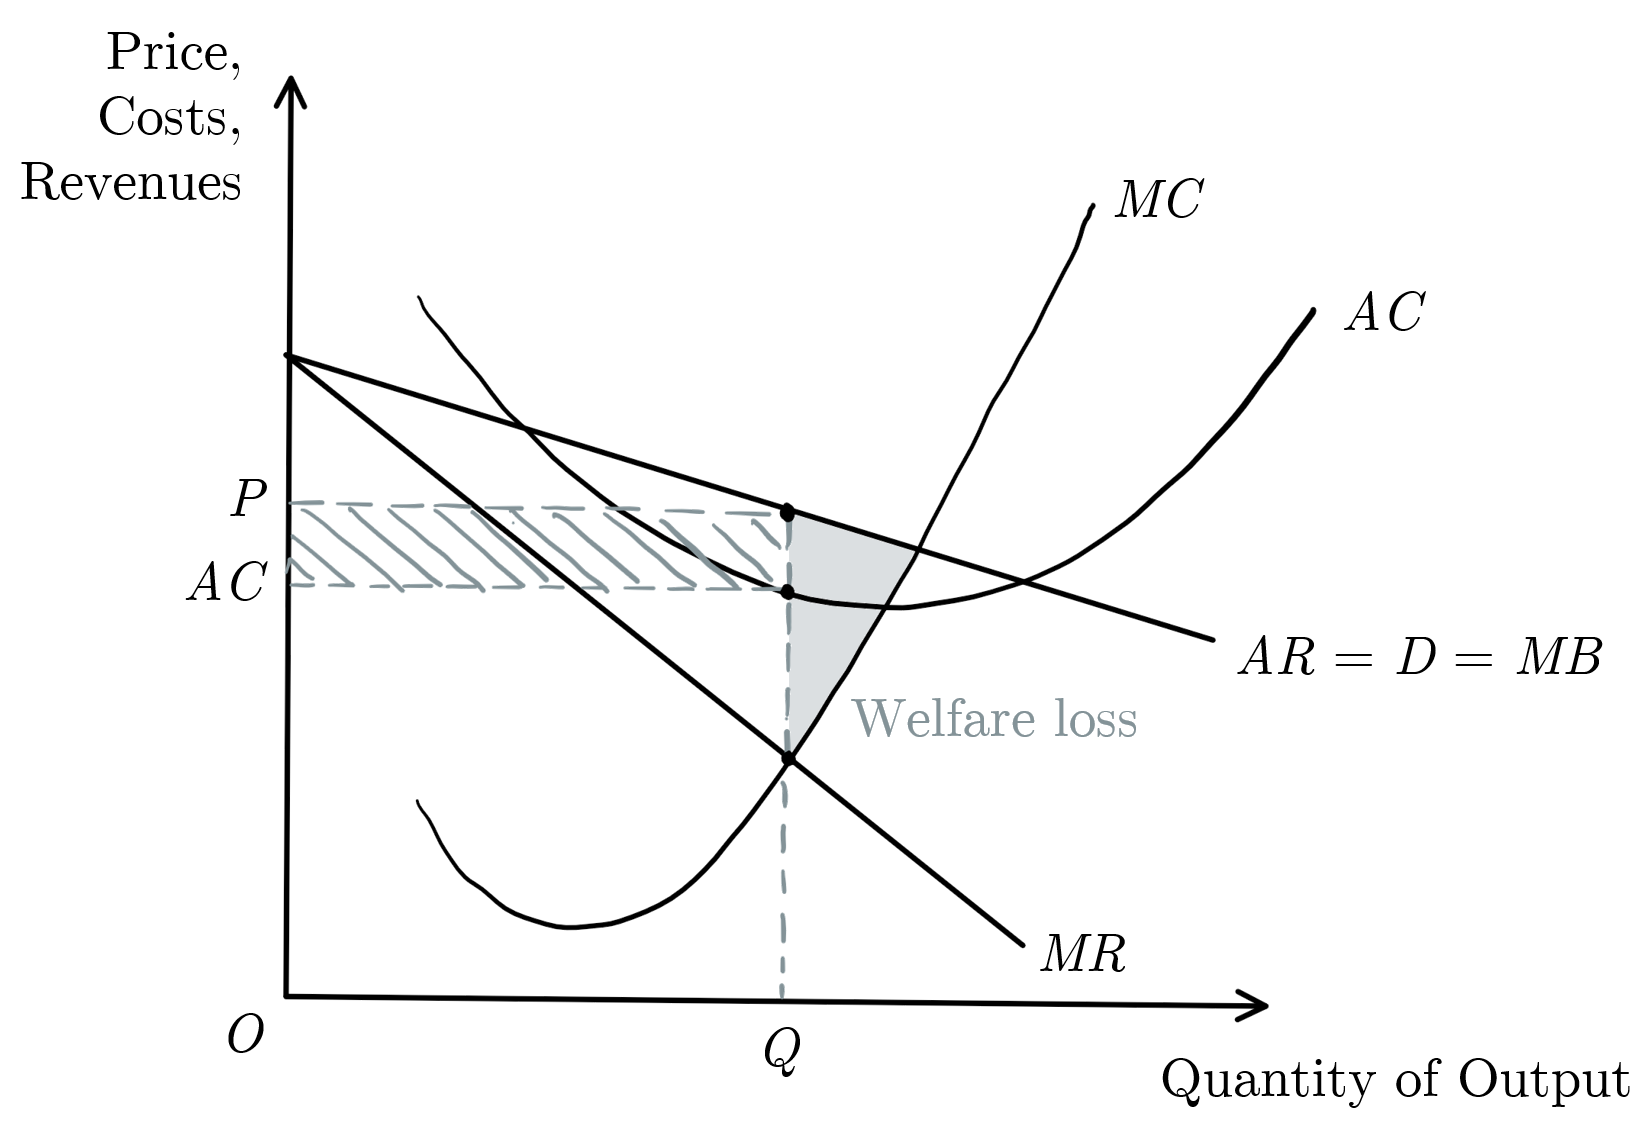
\includegraphics[width=0.6\linewidth]{monopoly.png}
	\caption{Allocative inefficiency due to abuse of market power by Alibaba}
	\label{fig:monopoly}
\end{figure}

\vspace{0.5cm}

The policy here is imposing a large fine, whose effect is shown in Figure~\ref{fig:fine}. As a result of the fine, Alibaba may decrease or stop its anti-competitive measures. This decreases its market power and shifts the demand curve to the left. Consequently, $MR$ also shifts to the left and intersects $MC$ at a lower quantity. The output is decreased from $Q$ to $Q$\textit{'}. The abnormal profit is also diminished from the light-gray-shaded region in the graph to the dark-gray-shaded region.

\begin{figure}[htbp]
	\centering
	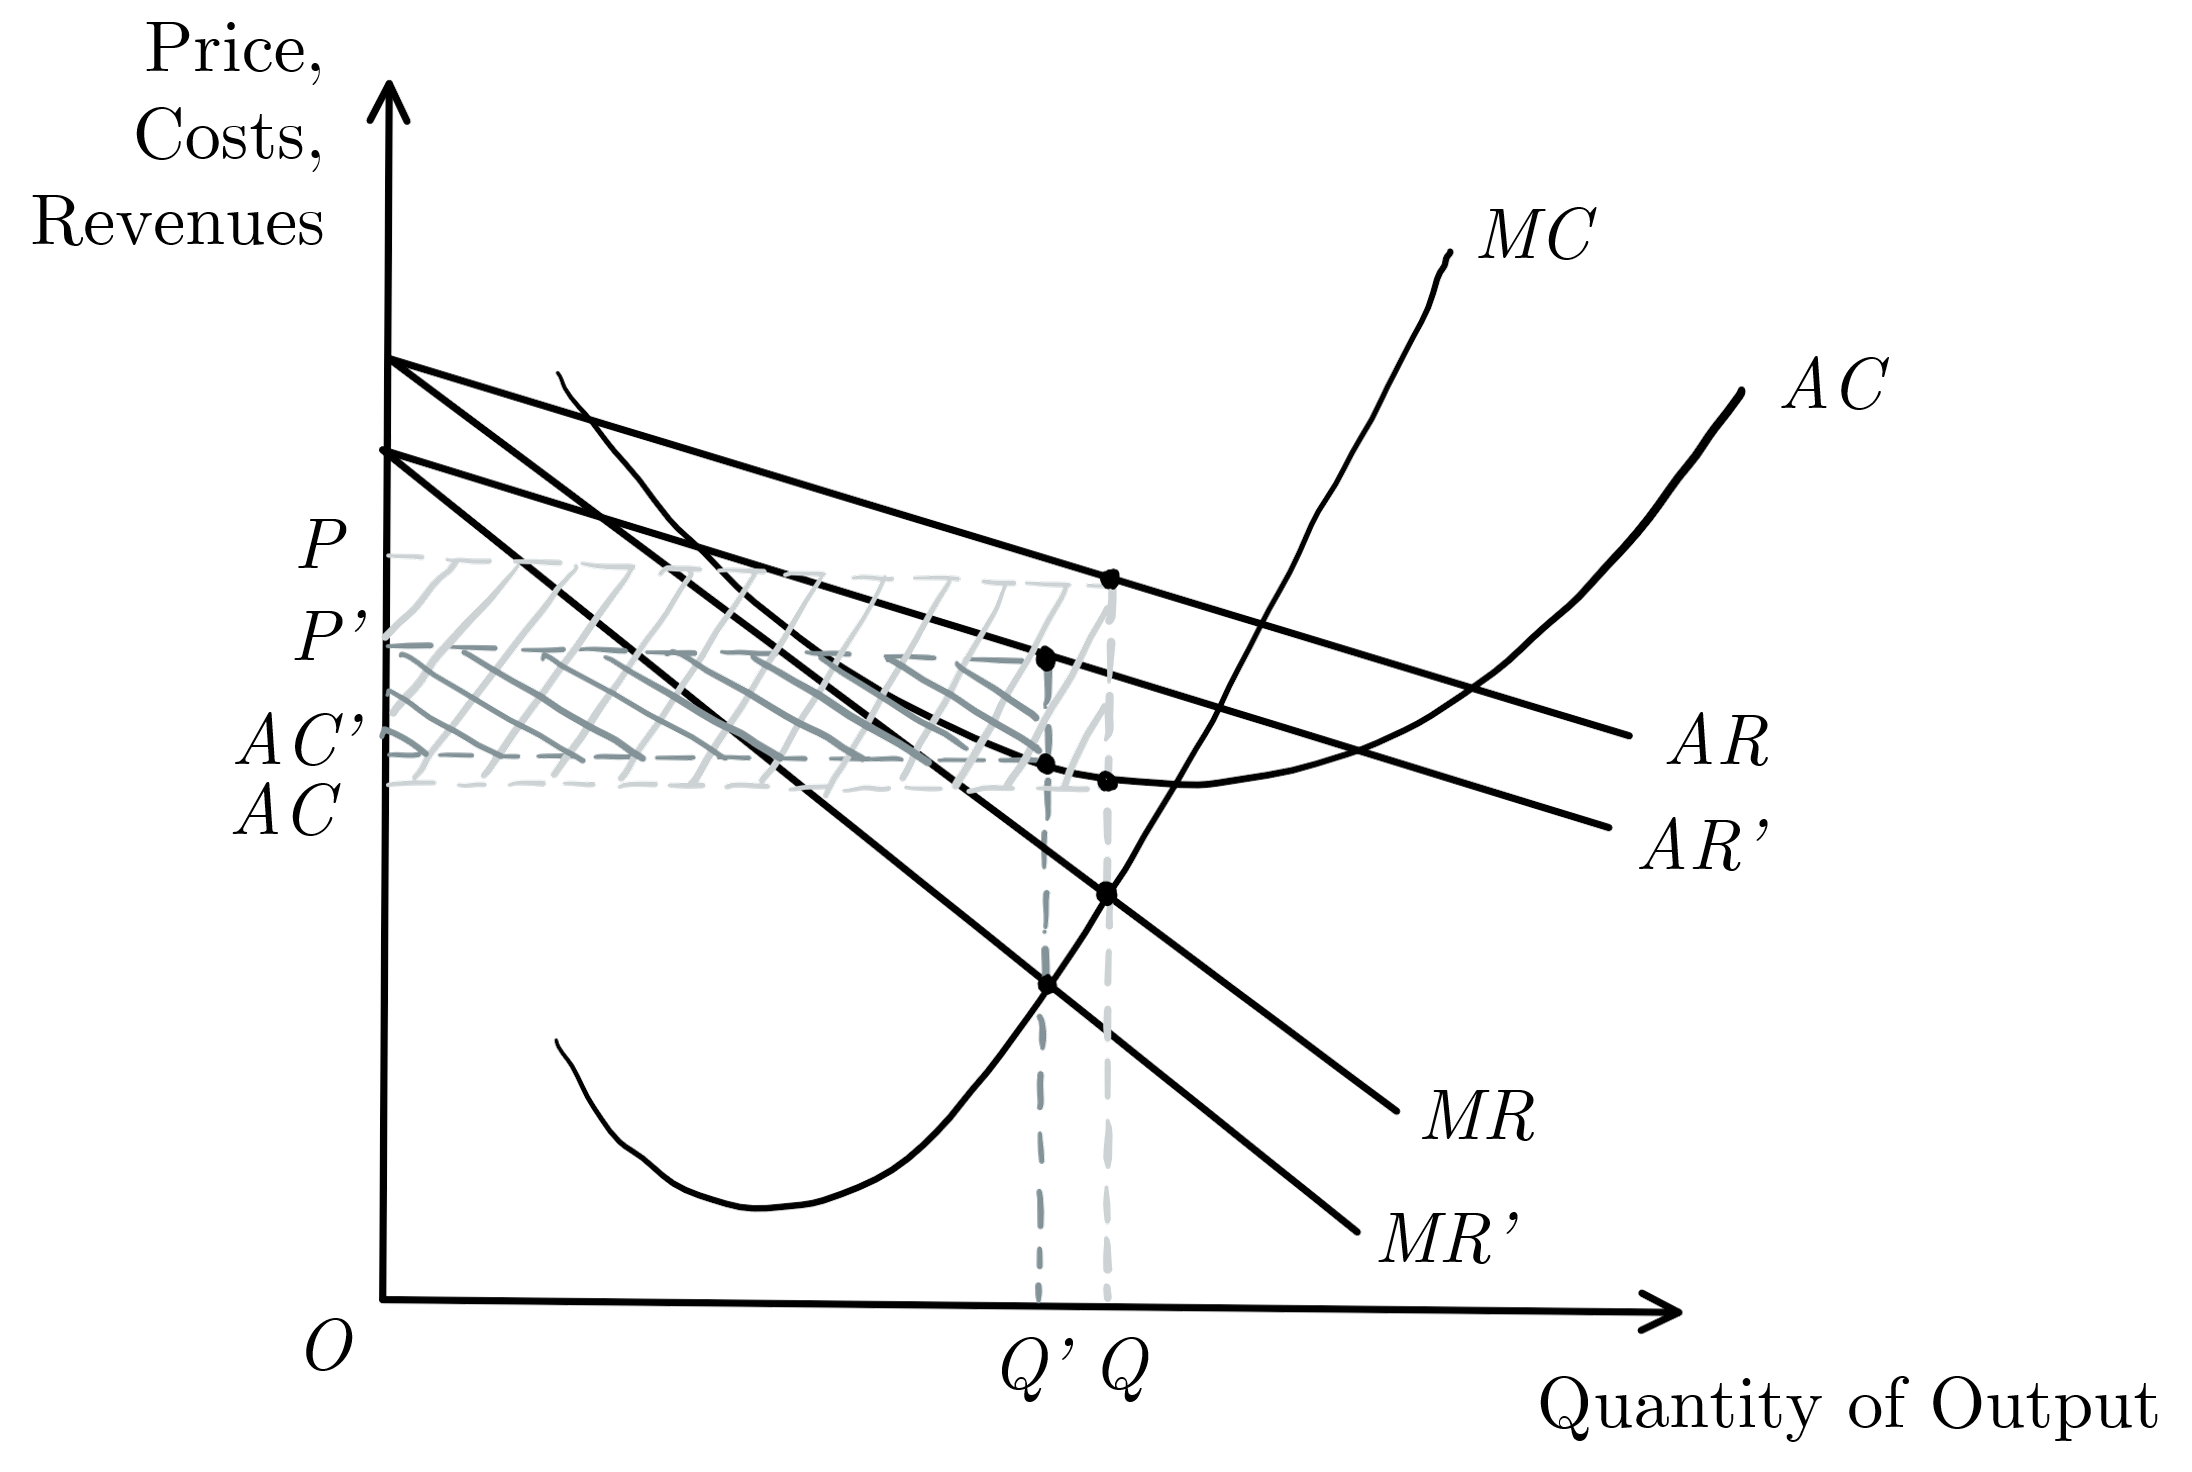
\includegraphics[width=0.6\linewidth]{fine.png}
	\caption{The mechanism of dealing with abuse of market power through fines}
	\label{fig:fine}
\end{figure}

\vspace{1cm}

There are several advantages and disadvantages to this approach.

One advantage is that this policy is straightforward and requires no continuous enforcement. Unlike legislation, which needs continued enforcement of the antitrust laws, fining only requires monitoring and subsequent penalizing the firms. The fine itself may be a sufficient incentive for Alibaba to stop its abuse of market power. 

Furthermore, the fine has an admonitory effect on other monopolists. Imposing this huge fine of \$2.8 billion can intimidate other firms that are undertaking similar anti-competitive measures and promote competition in other industries. 

However, the fines may be too small for a monopolist. Even though the fine is equal to 4\% of Alibaba's sales in China in 2019, Alibaba may still continue its practices if the profit from the anti-competitive practices can increase sales by more than 4\%. In other words,abusing market power may be too lucrative to successfully curb with fines.

Furthermore, Alibaba and similar monopolists may conceal some of their anti-competitive practices from government regulation. If so, then the government may find it hard to give out the deserved fines.


\end{document}